\documentclass{article}



\usepackage{graphicx,amsthm,amsmath,amssymb}
\graphicspath{ {./images/} }
\title{performance evaluation HW5}
\author{mina faridi }
\date{June 2022}
\begin{document}
\maketitle


	\nonumber \\
Question 1\\
\\
An approximation for the probability that you will make the wrong decision is $0.1587 .$
$S=N u m b e r$ of time that the result was odd
$$
\begin{aligned}
&n=100 \\
&p=0.5
\end{aligned}
$$
Hence:
$$
\begin{aligned}
&E[S]=100 \times 0.5 \\
&E[S]=50
\end{aligned}
$$
Standard deviation $=\sqrt{100} \times 0.5 \times 0.5$
Standard deviation $\sqrt{2} 5$
Standard deviation $=5$
Using normal approximation to the binomial
$$
\begin{aligned}
&\mathrm{P}(\mathrm{S} \geq 55)=\mathrm{P}(\mathrm{S}-50 / 5 \geq 55-50 / 5) \\
&\mathrm{P}(\mathrm{S} \geq 55)=1-\mathrm{P}(\mathrm{z} \leq 1) \\
&\mathrm{P}(\mathrm{S} \geq 55)=1-0.8413 \\
&\mathrm{P}(\mathrm{S} \geq 55)=0.1587
\end{aligned}
$$
Inconclusion an approximation for the probability that you will make the wrong decision is $0.1587 .$
(a) The sample size is computed using the central theorem.
For $95 \%$ confidence level, $z_{0.025}=1.96$. It is found in normal tables. Also the margin of error needs to be within $1 \mathrm{~cm}$. Thus,
$$
\begin{aligned}
n &=\left(\frac{\sigma \times z \frac{\alpha}{2}}{\mathrm{ME}}\right)^{2} \\
&=\left(\frac{1 \times 1.96}{1}\right)^{2} \\
&=3.8416 \\
& \cong 4
\end{aligned}
$$
At least 4 observations are needed.
(b) The chebyshev's inequality is as follows:
$$
p(|X-\mu| \geq \mathrm{ME}) \leq \frac{\sigma^{2}}{n \times \mathrm{ME}^{2}}
$$
So, the sample size formula is as follows:
$$
\begin{aligned}
n &=\frac{\sigma^{2}}{\alpha \times \mathrm{ME}^{2}} \\
&=\frac{1^{2}}{0.01 \times 5^{2}} \\
&=\frac{1}{0.25} \\
&=4
\end{aligned}
$$
Using the Chebyshev's inequality the samples size is tabulated, which need to be 4 to obtain the margin of error 5 with $99 \%$ confidence limit.
\\
\\
\\



	

Question 2: \\
\\

a. 
\\
$\mathrm{Y}_{\mathrm{1}}=\mathrm{X}_{\mathrm{1}} / \mathrm{1}$.\\
$\mathrm{Y}_{\mathrm{2}}=\mathrm{X}_{\mathrm{2}} / \mathrm{2}$.\\
$\mathrm{Y}_{\mathrm{3}}=\mathrm{X}_{\mathrm{3}} / \mathrm{3}$.\\
...\\
$\mathrm{Y}_{\mathrm{n}}=\mathrm{X}_{\mathrm{n}} / \mathrm{n}$.\\
we see that the denominator converges to infinite while the numerator is a limited number so the fraction converges to zero
\\

b.\\ $Y_{1}=\left(X_{1}\right)^{1}$\\
 $Y_{2}=\left(X_{2}\right)^{2}$\\
 $Y_{3}=\left(X_{3}\right)^{3}$\\
 ...\\
  $Y_{n}=\left(X_{n}\right)^{n}$\\
since n converges to infinity and the Base size is less than 1 so the deduction converges to zero

\\
c. \\
since all multiplications are less than one and the number of them is converging to infinity so the answer will converge to zero.
\\
d.\\ $\quad Y_{n}=\max \left\{X_{1}, \ldots, X_{n}\right\}$.\\
the more numbers we have, the probability of getting a number near to 1 increases and therefore the answer is 1.
\\





Question 3\\
	\\
	An approximation for the probability that you will make the wrong decision is $0.1587 .$
$S=N u m b e r$ of time that the result was odd
$$
\begin{aligned}
&n=100 \\
&p=0.5
\end{aligned}
$$
Hence:
$$
\begin{aligned}
&E[S]=100 \times 0.5 \\
&E[S]=50
\end{aligned}
$$
Standard deviation $=\sqrt{100} \times 0.5 \times 0.5$\\
Standard deviation $=\sqrt{2} 5$\\
Standard deviation $=5$\\
Using normal approximation to the binomial\\
$$
\begin{aligned}
&\mathrm{P}(\mathrm{S} \geq 55)=\mathrm{P}(\mathrm{S}-50 / 5 \geq 55-50 / 5) \\
&\mathrm{P}(\mathrm{S} \geq 55)=1-\mathrm{P}(\mathrm{z} \leq 1) \\
&\mathrm{P}(\mathrm{S} \geq 55)=1-0.8413 \\
&\mathrm{P}(\mathrm{S} \geq 55)=0.1587
\end{aligned}
$$
In conclusion an approximation for the probability that you will make the wrong decision is $0.1587 .$\\

\\

Question 4
\\
if we consider E[w]=0 (because of the fraction which the mean of its values equals to zero) then we should solve for p(|W|)<0.001\\
so the answer must be the area of this shape inside the square.\\
which equals to  (16*16 - (16-0.016)^2)/(16*16) = 0.19 \% \\


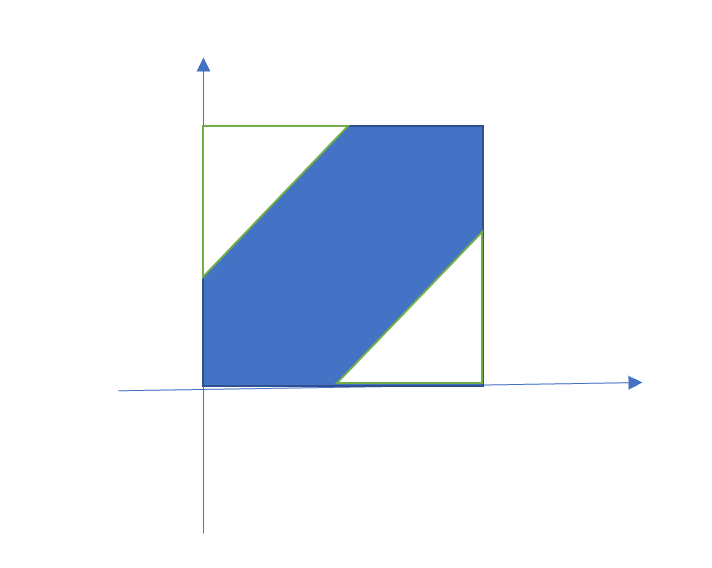
\includegraphics{images/1.png}
\\
\end{document}